	\documentclass{article}
\usepackage[colorlinks,citecolor=blue,urlcolor=blue]{hyperref}

\def\bbdot{\dot{\bb}}
\def\bgdot{\dot{\bg}}
\def\gdot{\dot{g}}
\def\ccdot{\dot{c}}
\def\adot{\dot{\ba}}
\def\bdot{\dot{\bb}}
\def\tdot{\dot{\bt}}
\def\tdd{\ddot{t}}
\def\addd{\ddot{a}}
\def\bdd{\ddot{b}}
\def\thetadot{\dot{\btheta}}
\def\covhat{\widehat{\cov}}
\def\siv{_{\text{IV}}}
\def\spp{_{\text{PP}}}
\def\sat{_{\text{AT}}}
\def\stsls{_{\text{TSLS}}}
\def\sps{_{\text{PS}}}
\def\saps{_{\text{APS}}}
\def\xpp{X\spp}
\def\sraw{_{s-\text{raw}}}
\def\sshrunk{_{s-\text{shrunk}}}
\def\ssplit{_{s-\text{split}}}
\def\thraw{\thetahat\sraw}
\def\thshr{\thetahat\sshrunk}
\def\thspl{\thetahat\ssplit}



\usepackage[margin=1in]{geometry}
\usepackage{lmodern}
\usepackage{amsmath}               
\usepackage{graphicx}

\usepackage[T1]{fontenc}
\title{Synthetic compliance estimation}
\RequirePackage{amsthm,amsmath,geometry,amsfonts}
\RequirePackage{natbib}
\usepackage[utf8]{inputenc}
\usepackage[english]{babel}
\usepackage{centernot}
\input{GrandMacros}
\input{Macro}

\newtheorem{assumption}{Assumption}
\begin{document}
\maketitle

\section{Introduction}
Noncompliance is common in studies with randomized assignments \textemdash ~some study subjects may self-select into a different study condition than their randomly assigned condition, hence breaking the orthogonality between study conditions and confounders.  Without further assumptions, the presence of noncompliance can downgrade a randomized experiment to a non-experimental study.  In pragmatic clinical trials, natural experiments, and quasi-experiments, a popular approach to circumvent the noncompliance issue is the intention-to-treat (ITT) analysis \citep{roland1998understanding, hollis1999meant, heckman2001policy}.  An ITT analysis aims to estimate a ``real-world'' or ``diluted'' effect of a treatment, ignoring the noncompliance in the study sample and assuming that the level of noncompliance in the study sample reflects the actual situation if the treatment were to be implemented elsewhere \citep{ten2008intent}.  The estimand in an ITT analysis is usually referred to as the \textit{effectiveness} of a treatment.  
An ITT analysis is straightforward for noncompliance, where the random assignments are used as the study factor and the actual treatment status subject to noncompliance are not considered.  Since the randomized assignment is orthogonal to all confounders, a simple two-sample comparison can be unbiased for estimating the effectiveness of a treatment \citep{angrist1999empirical, little2009comparison}. 

By contrast, the \textit{efficacy} of a treatment or the \textit{complier average causal effect} (CACE) refers to the mean causal effect among those who will always comply to randomized assignments, i.e., the \textit{principal compliers} \citep{angrist1996identification, little2009comparison}.  In the Economics literature, a favored approach to estimate the efficacy of a treatment is a structural equation model, where the randomized assignment is considered as an instrument variable (IV) for the actual treatment status \citep{greene2003econometric}.  Under certain assumptions, the IV approach is unbiased for estimating the efficacy of a treatment.   See \citep{imbens2014instrumental} for a detailed survey of methods and development in this space. Despite its popularity, the IV approach can have a high variance, particularly if the sample proportion of principal compliers is low \citep{little2009comparison, antonelli2017synthetic}.
 	
Two different approaches, the per-protocol (PP) and as-treated (AT) analyses, have also received many applications \citep{higgins2008cochrane, mcnamee2009intention}. The per-protocol (PP) analysis subsets the sample to those whose actual treatment statuses are the same as their randomized assignments, i.e., \textit{observed compliers}.  However,  observed compliers are usually different from principal compliers. For example, those who would always refuse a treatment, i.e., \textit{never-takers}, cannot be differentiated from principal compliers when randomized to the control condition.  The difference between the observed and principal compliers results in biases in the PP analysis. By contrast, the as-treated (AT) analysis ignores the initial assignment and uses the actual treatment to estimate a treatment effect.  Due to various sample selection biases, the AT analysis can be severely biased.  Despite their biases, both the PP and AT analyses usually have a smaller estimation variance than the IV approach.  If we measure the efficiency of an estimator by its mean squared error (MSE), i.e., the sum of its squared bias and sampling variance, among IV, PP, and AT estimators, none can always outperform the others.  See, e.g., \citep{little2009comparison, antonelli2017synthetic}, for discussions of the scenarios where each estimator can outperform the others.  The suitable scenario for each estimator depends on non-estimable properties of some unobserved data, e.g., whether there is a mean difference in the outcome between non-takers and principal compliers when randomized to the control condition.  

In this paper, we consider a synthetic estimator as a convex combination of the IV, AT, and PP estimators (referred to as the candidate estimators, hereafter).  
Our approach is rooted in the theory of model averaging, which conventionally focuses on estimating coefficients in least square regression models (see \citep{buckland1997model, hjort2003frequentist, judge2004semiparametric, mittelhammer2005combining, longford2006missing, hansen2007least} as prominent examples) and predicting random effects in mixed-effect models \citep{robinson1991blup, ghosh1994small, Searle1997, longford2006missing}. We use the term synthetic estimation instead of model averaging because our candidate estimators do not belong the same class of models, although they target the same estimand of interest, i.e., the CACE.

One purpose of synthetic estimation is to combine several available candidate estimators to form a single and unambiguous estimator.  In addition, by striking a balance between biases and variances, a combination of candidate estimators can have a smaller MSE than all candidate estimators. The theoretical framework of model-averaging is much wider than linear regression and mixed-effect models.  In the recent literature, \citep{lavancier2016general} outlined synthetic estimators for a very general class of problems and provide some asymptotic results. \citet{antonelli2017synthetic} proposed a synthetic estimator in the presence of non-compliance in the setting of a randomized controlled trial.  

In the spirit of \citet{antonelli2017synthetic}, we propose a class of synthetic compliance estimators (SCE) which optimally combine candidate estimators of the CACE by minimizing the estimated MSE of the resulting estimator. The proposed SCE are appropriate for observational studies, and other non-experimental studies where covariates must be adjusted for in the estimation.  The SCE display a robustness property: without sacrificing too much on the estimation bias, it borrows information from other biased but precise candidate estimators to improve the overall efficiency estimation as measured by MSE. 

The rest of the paper is organized as follows. In Section 2, we outline specifics about the principal compliance framework and lay out the details of the candidate estimators in this setting. In Section 3, we present the SCE and their practical implementation. The asymptotic property of the SCE is discussed in Section 4.  Section 5 includes simulations demonstrating the robustness of the SCE. In Section 6 we apply the SCE to analyze a natural experiment. Section 7 contains concluding remarks.


\section{Framework}
Suppose interest lies in the effect of a treatment $S_i$ on an outcome $Y_i$ and there exists a pre-treatment instrument $Z_i$, such as allocation to treatment, for $n$ subjects indexed by $i$. Further, suppose $\bX_i$ is a set of covariates collected on these $n$ subjects. We assume throughout that $Z_i$ and $S_i$ are binary, so that they take values in $\{0, 1\}$. Let $S_i(z)$ be the treatment status that, possibly contrary to fact, would have been observed if $Z_i = z, z = 0, 1$. Based on the configuration of these counterfactuals, there are potentially four types of individuals in the population: \textit{always-} and \textit{never-takers} who are not influenced by the instrument and for whom $S_i(z) = 1$ (always-takers) or $S_i(z) = 0$ (never-takers), $z = 0, 1$; \textit{compliers} who take treatment according to the instrument $S_i(z) = z$; and \textit{defiers} who do the opposite of the instrument $S_i(z) = 1 - z$. Let $\pi_c = P(S_i(0) = 0, S_i(1) = 1)$ be the probability of being a complier. 

Further define the counterfactual outcome $Y_i(z, s)$ to be the outcome that one would observe if, possibly contrary to fact, $Z_i = z$ and $S_i = s$. For these counterfactuals to make sense, we assume the no-interference or Stable Unit Treatment Value Assumption (SUTVA) holds \citep{rubin1978bayesian} for both the potential outcomes $Y_i(z,s)$ and the potential treatments $S_i(z)$. That is, that the potential outcomes and potential treatment values for individual $i$ do not depend on any other individual, and $S_i = S_i(1)Z_i + S_i(0)(1-Z_i)$ and 
\begin{align*}
    Y_i = Y_i(1, 1)Z_iS_i + Y_i(0, 1)(1-Z_i)S_i + Y_i(1, 0)Z_i(1-S_i) + Y_i(0, 0)(1-Z_i)(1-S_i).
\end{align*} 

\subsection{The estimand}
Typically, the effect of most interest is the average treatment effect (ATE), $E[Y_i(1) - Y_i(0)]$, where $Y_i(s)$ is the counterfactual outcome that would have been observed if $S_i = s$. However, in many situations the ATE is not identifiable due to failure to measure all variables that confound the relationship between $S_i$ and $Y_i$ in $\bX_i$, so that 
\[
\{Y_i(0), Y_i(1)) \centernot\amalg S_i | \bX_i.
\]
In these cases, especially in studies where $Z_i$ is randomized such as in clinical drug trials, it is typical to estimate the so-called intention-to-treat (ITT) effect, or $E[Y_i | Z_i = 1] - E[Y_i | Z_i = 0]$, which is equivalent to the causal effect of treatment assignment when $Z_i$ is randomized, $E[Y_i(1, S_i(1)] - E[Y_i(0, S_i(0)]$. This effect is sometimes called \textit{treatment effectiveness}, but it does not tell us about the effect of $S_i$, or treatment \textit{efficacy}. 

To get at treatment efficacy, the local average treatment effect \citep{Angrist1995} or the complier average causal effect (CACE) \citep{little2009comparison} may instead be selected as the target of estimation. The CACE is the causal effect among those whose receipt of treatment is affected by the instrument: 
\begin{align}
\theta = E\{Y_i(1) - Y_i(0) | S_i(0) = 0, S_i(1) = 1\}. \label{cace}
\end{align}
We note here that the CACE is instrument-dependent - a different instrument would yield a different estimand of treatment efficacy. Because of this and other difficulties with identifying compliers, some \citep{} question the use of the CACE as an estimand. While others are  We acknowledge this debate but start from the assumption that the CACE is a worthwhile target. If a different estimand were preferred, much of our development below would still be useful in improving estimation of the new estimand.


\subsection{Identifying assumptions}
In this section, we outline a series of assumptions that are typically used to identify the CACE. Some estimators will require all of the ensuing assumptions, and some estimators may require only a few. 
\begin{assumption}[Pseudo-randomization] \label{iv_randomized}
    \begin{align*}
    \left.Z_i \amalg \left\{S_i(0), S_i(1), Y_i(0, 0), Y_i(0, 1), Y_i(1, 0), Y_i(1, 1)\right\}\right|\bX_i.    
    \end{align*}
\end{assumption}
Assumption \ref{iv_randomized} states that the instrument is, if not randomized, as good as randomized \citep{imbens2014instrumental} within strata defined by the covariates $\bX_i$. This assumption is similar in spirit to the no-unmeasured-confounders assumption commonly invoked for treatment effect estimation. 

\begin{assumption}[Exclusion restriction]\label{er}
\begin{align*}
    E[Y_i(0, s)] = E[Y_i(1, s)], s = 0, 1 \label{er}
    \end{align*}
\end{assumption} 
Assumption \ref{er} encodes the so-called exclusion restriction (ER), which states that there is no direct effect of the treatment assignment on the outcome in the population. A stronger version of the ER states the equality at the individual-level and ensures there is a single counterfactual outcome for each treatment: $Y_i(s) = Y_i(0, s) = Y_i(1,s)$. In situations where the instrument is an indicator of double-blind randomization, the ER is very plausible. In other cases, it must be justified based on substantive expertise. 

We further may require a stronger assumption the effect of compliance:
\begin{assumption}[No compliance effect]\label{nce}
\begin{align*}
    E[Y_i(z, s) | S_i(0) = 0, S_i(1) = 1, \bX_i] = E[Y_i(z, s) | S_i(0) = z, S_i(1) = z, \bX_i], z = 0, 1; s = 0, 1. 
    \end{align*}
\end{assumption}
Assumption \ref{nce} is not needed for traditional IV estimators or two-stage least squares estimators. This assumption states that compliers ($S_i(0) = 0, S_i(1) = 1$) have the same outcomes as non-compliers and thus there is \textit{no compliance effect} (NCE) either when $Z_i = 0$ or $Z_i = 1$. This assumption was termed General Principal Ignorability  in \cite{Ding2017}.

Finally, we will make two monotonicity assumptions. The first is required for identifiability and states that there are no defiers in the population and the treatment assignment does not make anyone less likely to take treatment:
\begin{assumption}[Monotonicity]\label{monotonicity}
\begin{align*}
S_i(0) \leq S_i(1). 
\end{align*}
\end{assumption}
The second is purely for ease of presentation:
\begin{assumption}[Strong monotonicity]\label{strong_monotonicity}
\begin{align*}
S_i(0) = 0. 
\end{align*}
\end{assumption}
This second stronger version of monotonicity ensures that there are no always-takers ($S_i(0) = 1, S_i(1) = 1$). While strong monotonicity may not be a reasonable assumption in all cases, any additional complexity arising due to its violation (by inclusion of always-takers) could easily be incorporated in the framework we lay out here. 

%It is typical to assume that there are no defiers in the population, and in some situations where patients do not have independent access to the treatment, always-takers may be assumed away as well. Both are ensured by the so-called strong monotonicity assumption which can be found in \citep{Ding2017}:

%\begin{assumption}\label{strong_monotonicity}
%Strong monotinicity. \[
%S_i(0) = 0
%\]
%\end{assumption}

%Define the complier average causal effect (CACE) to be $$\theta = E\{Y_i(1) - Y_i(0) | \bU_i = (0,1)\}.$$ Define also the principle score to be $e(\bx) = P(\bU_i = (0,1) | \bX_i = \bx)$. Define similar but unconditional quantities $\pi_{11} = P(\bU_i = (1,1) | Z_i = 0)$ and $\pi_{00} = P(\bU_i = (0,0) | Z_i = 1)$. Let $n_0 = \sum_{i=1}^n I\{Z_i = 0\}$ and $n_1 = \sum_{i=1}^n I\{Z_i = 1\}$ be the treatment assignment sample sizes, and let $\ntilde_0 = \sum_{i=1}^n I\{S_i = 0\}$ and $\ntilde_1 = \sum_{i=1}^n I\{S_i = 1\}$ be the actual observed treatment sample sizes.

% \subsection{Assumptions}

% In this section we lay out various assumptions that may be used to justify various estimators of the CACE. These assumptions are adapted from \citep{Little2018} and \citep{Ding2017}. 

% \begin{assumption}[SUTVA]\label{sutva}
% Stable unit treatment value assumption.
% \end{assumption}

% \begin{assumption}\label{randomization}
% Randomization. 
% \[
% Z_i \amalg \left\{S_i(0), S_i(1), Y_i(1), Y_i(0), \bX_i\right\}
% \]
% \end{assumption}

% \begin{assumption}\label{monotonicity}
% Monotinicity. \[
% S_i(1) \geq S_i(0)
% \]
% \end{assumption}

% \begin{assumption}\label{strong_monotonicity}
% Strong monotinicity. \[
% S_i(0) = 0
% \]
% \end{assumption}

% \begin{assumption}[NCEC]\label{ncec}
% No compliance effect among the controls. %\[Y_i(0) \amalg \bU_i | U_{i1} = 0, Z_i = 0, \bX_i\]
% \[
% E[Y_i(0) | \bU_i = (0, 1)] = E[Y_i(0) | \bU_i = (0, 0)]
% \]
% \end{assumption}
% Note that Assumption \ref{ncec} is labeled NCEC$_\mu$ in \citep{Little2018}, while a stronger version is labeled NCEC:  $Y_i(0) \amalg \bU_i | U_{i1} = 0, Z_i = 0$. We stick with the weaker assumption on expectations here. 



% \begin{assumption}[Conditional NCEC v2]\label{cncec2}
% No compliance effect among the controls conditional on never-taker principal score $e\{(0,0); \bX_i\}$. %\[Y_i(0) \amalg \bU_i | U_{i1} = 0, Z_i = 0, \bX_i\]
% \[
% E[Y_i(0) | \bU_i = (0, 1), e\{(0,0); \bX_i\}] = E[Y_i(0) | \bU_i = (0, 0), e\{(0,0); \bX_i\}]
% \]
% \end{assumption}

% \begin{assumption}[NCET]\label{ncet}
% No compliance effect among the treated. %\[Y_i(1) \amalg \bU_i | U_{i2} = 1, Z_i = 1, \bX_i\]
% \[
% E[Y_i(1) | \bU_i = (0, 1)] = E[Y_i(1) | \bU_i = (1, 1)]
% \]
% \end{assumption}



% \begin{assumption}[ER]\label{er}
% Exclusion restriction. 
% \[
% %\left\{Y_i(0), Y_i(1)\right\} \amalg Z_i | \bU_i = (0, 0), \bX_i; \qquad
% %\left\{Y_i(0), Y_i(1)\right\} \amalg Z_i | \bU_i = (1, 1), \bX_i
% E[Y_i(0) | \bU_i = (0, 0)] = E[Y_i(1) | \bU_i = (0, 0)]; \qquad
% E[Y_i(0) | \bU_i = (1, 1)] = E[Y_i(1) | \bU_i = (1, 1)]
% \]
% \end{assumption}

% % \begin{assumption}[Conditional ER]\label{cer}
% % Exclusion restriction conditional on $\bX_i$. 
% % \[
% % %\left\{Y_i(0), Y_i(1)\right\} \amalg Z_i | \bU_i = (0, 0), \bX_i; \qquad
% % %\left\{Y_i(0), Y_i(1)\right\} \amalg Z_i | \bU_i = (1, 1), \bX_i
% % E[Y_i(0) | \bU_i = (0, 0), \bX_i] = E[Y_i(1) | \bU_i = (0, 0), \bX_i]; \qquad
% % E[Y_i(0) | \bU_i = (1, 1), \bX_i] = E[Y_i(1) | \bU_i = (1, 1), \bX_i]
% % \]
% % \end{assumption}

% \begin{assumption}[PI]\label{pi}
% Principal ignorability.
% \[
% Y_i(0) \amalg \bU_i | \bX_i
% \]
% \end{assumption}
% Note that this may(?) be a stronger assumption than the stronger version of Assumption \ref{ncec}. 

% \begin{assumption}[GPI]\label{gpi}
% Generalized principal ignorability.
% \[
% Y_i(0) \amalg \bU_i | \bX_i; \qquad Y_i(1) \amalg \bU_i | \bX_i
% \]
% \end{assumption}

% % \begin{assumption}
% % Stratification sufficiency. 

% % \end{assumption}


\subsection{Candidate CACE estimators}
For clarity and ease of presentation, we restrict ourselves to a series of well-known estimators for the CACE. The SCE could easily be adapted to include other candidate estimators with ease. 

\paragraph{IV estimator.} The first is the standard IV estimator
\begin{align}
    \thetahat\siv = \frac{n_1\inv\sum_{i=1}^nY_iI\{Z_i = 1\} - n_0\inv\sum_{i=1}^nY_iI\{Z_i = 0\}}{\pihat_c}. \label{iv_est}
\end{align}
Under assumptions \ref{iv_randomized}, \ref{er}, and \ref{monotonicity}, $\thetahat\siv$ is consistent for the CACE, and under assumption \ref{strong_monotonicity}, $\pihat_c = \Phat(S_i(0) = 0, S_i(1) = 1)$ may be estimated by $n_1\inv\sumin I\{S_i = 1 | Z_i = 1)$, with $n_z$ equal to the sample size with instrument value $Z_i = z$.

\paragraph{Two-stage least squares.} The second is the two-stage least squares estimator of \cite{Angrist1995}, where the CACE is estimated as $\thetahat_{TSLS} = \thetahat$ from the model
\begin{align}
    Y_i = \beta_0 + \theta \Shat_i + \bgamma\trans\bX_i + \epsilon_i, i = 1, ..., n
\end{align}
and $\Shat_i$ is the predicted value of a regression of $S_i$ onto $\bX_i$. Under assumptions \ref{iv_randomized}, \ref{er}, \ref{monotonicity}, and assuming the models for $Y_i$ and $S_i$ are correct, $\thetahat\stsls$ is consistent for the CACE.

\paragraph{Per-protocol.} We further consider a \textit{per-protocol} estimator, where we use a model-based estimator for the effect of receiving the treatment among those individuals whose treatment and instrument agree. The PP estimator is found as $\thetahat\spp = \thetahat$ from the model:
\begin{align}
    Y_i = \beta_0 + \theta S_i + \bgamma\trans\bX_i + \epsilon_i, i \in \{j : S_j = Z_j\}.\label{pp-model}
\end{align}
Under assumptions \ref{iv_randomized}, \ref{nce} and \ref{monotonicity}, and assuming the model \eqref{pp-model} holds, $\thetahat\spp$ is consistent for the CACE. 

\paragraph{As-treated.} We also consider an \textit{as-treated} estimator, where the instrument is ignored, and we simply estimate the effect of $S_i$ from a model. It is found as $\thetahat\sat = \thetahat$ from the model:
\begin{align}
    Y_i = \beta_0 + \theta S_i + \bgamma\trans\bX_i + \epsilon_i, i = 1, ..., n \label{at-model}
\end{align}
Under assumptions \ref{iv_randomized}, \ref{er}, \ref{nce} and \ref{monotonicity}, and assuming the model \eqref{at-model} holds, $\thetahat\sat$ is consistent for the CACE.

\paragraph{Principal-score weighting estimators.} We also consider weighting methods using so-called principal scores that are laid out in \cite{Ding2017}. The principle score for compliers or compliance score is $e(\bX) = P(S_i(0) = 0, S_i(1) = 1 | \bX),$ the probability of being a complier. We consider two principal-score estimators. The first is purely a weighting estimator and can  be written:
\begin{align}
    \thetahat\sps = n_{11}\inv\sum_{i : S_i = 1, Z_i = 1} Y_i - n_0\inv\sum_{i : Z_i = 0} \frac{Y_i\ehat(\bX_i)}{\Phat(S_i(0) = 0, S_i(1) = 1)}.
\end{align}
Under assumptions \ref{iv_randomized}, \ref{nce} and \ref{strong_monotonicity}, $\thetahat\sps$ is consistent for the CACE. 

The second estimator is a model-assisted version of the same estimator:
\begin{align}
    \thetahat\saps &= n_{11}\inv\sumin (Y_i - \bbetahat_1\trans\bX_i)I\{S_i = 1, Z_i = 1\} - n_{0}\inv\sumin \frac{(Y_i - \bbetahat_0\trans\bX_i)\ehat(\bX_i)I\{Z_i = 0\}}{\Phat(S_i(0) = 0, S_i(1) = 1)} +\\
    &\qquad (n_0 + n_{11})\inv\sumin \frac{(\bbetahat_1 - \bbetahat_0)\trans\bX_i\ehat(\bX_i)I\{Z_i = 0 \text{ or } S_i = 1, Z_i = 1\}}{\Phat(S_i(0) = 0, S_i(1) = 1)}
\end{align}
where $n_{zs}$ is the sample size in group $Z_i = z, S_i = z$ and $\bbetahat_1$ is estimated from the model
\[
Y_i = \beta_0 + \bbeta_1\trans\bX_i + \epsilon_i, i \in \{j : S_j = 1, Z_j = 1\}
\]
and $\bbetahat_0$ is estimated from the model
\[
Y_i = \beta_0 + \bbeta_1\trans\bX_i + \epsilon_i, i \in \{j : Z_j = 0\}.
\]
Under assumptions \ref{iv_randomized}, \ref{nce} and \ref{strong_monotonicity} -- no additional assumptions from $\thetahat\sps$ -- $\thetahat\saps$ is consistent for the CACE and has a lower asymptotic variance.
\paragraph{Principal-score stratified estimators.} We finally estimate versions of the IV, AT, and PP estimators that are stratified by the principal score. We first estimate each estimator withiin quintiles of the principal score and then averaged across quintiles. We will denote these estimators as $\thetahat_{IVs}, \thetahat_{PPs}, \thetahat_{ATs}$. 

\subsection{Some properties of candidate estimators}


% \paragraph{Vanilla IV.} Under Assumptions \ref{strong_monotonicity}, \ref{sutva}, and \ref{er}, the following estimator is consistent for the CACE \[
% \thetahat\siv(0, 1) = \frac{n_1\inv\sum_{i=1}^nY_iI\{Z_i = 1\} - n_0\inv\sum_{i=1}^nY_iI\{Z_i = 0\}}{1 - \pihat_{00}}
% \]
% provided that $\pi_{00}$ is estimated consistently. The exclusion restriction guarantees that the instrument has no effect on the mean counterfactual outcome in the never-takers. 

% In a similar vein, we can propose a model-based two-stage least squares estimator, where we first regress $S_i$ onto $\bX_i$ in the treated group (does this require strong monotonicity?). Then, we obtain a prediction for $S_i(\bX_i)$ among all subjects, which we call $\Shat(\bX_i)$, and then regress $Y_i$ onto $\Shat(\bX_i)$ and $\bX_i$.

% \paragraph{Two-stage least squares.} Under Assumptions \ref{strong_monotonicity}, \ref{sutva}, and \ref{er}, the coefficient corresponding to $\Shat(\bX_i)$ in a regression of $Y_i$ onto $\Shat(\bX_i)$ and $\bX_i$ will be consistent for the CACE as long as $\Shat(\bX_i) \rightarrow P(S_i = 1 | \bX_i)$ and the regression model is correctly specified.  

% We also consider two other assumptions and estimators. 

% \begin{assumption}[Conditional NCET]\label{cncet1}
% No compliance effect among the treated conditional on $\bX_i$. 
% \[
% E[Y_i(1) | \bU_i = (0, 1), \bX_i] = E[Y_i(1) | \bU_i = (1, 1), \bX_i]
% \]
% \end{assumption}

% \begin{assumption}[Conditional NCEC]\label{cncec1}
% No compliance effect among the controls conditional on $\bX_i$. %\[Y_i(0) \amalg \bU_i | U_{i1} = 0, Z_i = 0, \bX_i\]
% \[
% E[Y_i(0) | \bU_i = (0, 1), \bX_i] = E[Y_i(0) | \bU_i = (0, 0), \bX_i]
% \]
% \end{assumption}

% These assumptions give rise to the per-protocol estimator:
% \paragraph{Conditional per-protocol.} Under Assumptions \ref{sutva}, \ref{cncec1} and \ref{cncet1}, the coefficient corresponding to $S_i$ from a regression of $Y_i$ on $S_i$ and $\bX_i$ among patients for whom $S_i = Z_i$ will be consistent for the CACE as long as the regression model is correctly specified. 

% A final estimator invokes both the exclusion restriction and NCEC/NCET:
% \paragraph{Conditional as-treated.} Under Assumptions \ref{sutva}, \ref{cncec1}, \ref{cncet1}, and \ref{er} the coefficient corresponding to $S_i$ from a regression of $Y_i$ on $S_i$ and $\bX_i$ will be consistent for the CACE as long as the regression model is correctly specified. 

\section{Synthetic estimation}



In this section, we propose a class of SCE which leverages the information in all candidate estimators. 
Let the set of candidate estimators be denoted as $\bthetahat = (\thetahat_0, \thetahat_1, ..., \thetahat_k)' = (\thetahat_0, \bthetahat_1')'$, where $\thetahat_0$ is an estimator that can be presumed to be unbiased, and $\bthetahat_1$, a vector of length $k$, collects all other candidates.  Because the exclusion restriction (\ref{er}) can often be plausibly assumed to hold, we typically consider either the vanilla IV estimator or the TSLS estimator to be $\thetahat_0$.  When the assumption (\ref{er}) is deemed unlikely, another estimator may be considered as $\thetahat_0$. We consider a synthetic estimator as a convex combination of the candidates \[
\bb'\bthetahat = b_0\thetahat_0 + \bb_1'\bthetahat_1
\]
where all entries of $\bb'$ are between 0 and 1, and sum to 1. 

The synthetic estimator aims to lower the MSE of the supposedly unbiased $\theta_0$ by including the possibly biased $\bthetahat$ in the hopes of attaining lower variance without overly sacrificing on the estimation bias.  To achieve this goal, the convex combination $\bbtilde$ would ideally be chosen to directly minimize the MSE.  We adopt the same rationale in \citep{robinson1991blup, longford2006missing} to derive the SCE. Specifically, 
let the sampling variance of the candidate estimators be
\begin{equation}
\Sigma = \var \begin{pmatrix} \hat\theta_0 \\ \boldsymbol {\hat\theta}_1  \end{pmatrix} =
\begin{pmatrix}     V_{0,n} & \mathbf C'_n\\
                             \mathbf C_n     & \mathbf V_n \end{pmatrix},
\end{equation}
where the small $n$ in the subscript denotes the finite sample size. 
Let the biases of candidate estimators be denoted as
\begin{equation}\begin{split}
    &\mathbf d_n = E(\boldsymbol {\hat\theta} - \theta) = (d_{0,n}, \mathbf d_n')'
\end{split}\end{equation}
Given $\bb$, the plug-in estimation for the MSE of $\bb'\bthetahat$ is
\begin{equation}\begin{split}\label{bMSE}
 &\quad E[( \bb'\bthetahat - \theta)^2]  \\
	&= (1 - \mathbf 1' \mathbf b)^2  (\hat d_{0,n}^2+ \hat V_{0,n}) + \mathbf {b' \hat V}_n \mathbf b  + 2 (1-\mathbf{1'b} )(\mathbf{\hat C}'_n + \hat d_{0,n}\hat{\mathbf d}'_n ) \mathbf{b} + (\mathbf{b'}\hat{\mathbf{d}}_n)^2  \\
    &= \hat d_{0,n}^2 + \hat V_{0, n} - 2(\mathbf P_n + \hat d_{0,n}^2-\hat d_{0,n}\hat{\mathbf d}_n)' \mathbf b + \mathbf b'(\mathbf T_n + \mathbf D_n )\mathbf b,
\end{split}\end{equation}
where the hat symbol denotes an estimator for the corresponding sampling moment and 
\begin{displaymath}\begin{split}
&\mathbf P_n = P_n(\Sigmahat) =\hat V_{0, n} - {\mathbf{\hat C}}_n, \\
&\mathbf T_n= T_n(\Sigmahat) = \hat V_{0,n} - \mathbf{1 \hat C'}_n - \mathbf{\hat C}_n \mathbf{1'} + \mathbf{\hat V}_n, \\
&\mathbf D_n = D_n(\bdhat_n) = \hat{\mathbf{d}}_n \hat{\mathbf{d}}_n' +\hat d_{0,n}^2 -2\hat d_{0,n}\mathbf 1\hat{\mathbf d}'_n,
\end{split}\end{displaymath}

Let $\mathbf b^*$ be the minimizer of \eqref{bMSE}, which is a typical problem of constrained quadratic programming. Suppose $\mathbf b^*$ is not on the boundary of the convex constraint. Then, 
\begin{equation} \label{eqn:opt}
\mathbf b^* = b^*(\bdhat_n, \Sigmahat) = (\mathbf T_n + \mathbf D_n)^{-1}(\mathbf P_n +\hat d_{0,n}^2 -\hat d_{0,n}\hat{\mathbf d}_n).
\end{equation}
If $\mathbf b^*$ is out of the boundaries, \eqref{eqn:opt} needs to be projected to the boundaries of the convex constraints.  

Our proposed SCE has the following general form
\begin{equation}
\hat\theta_s = (1-\mathbf 1'\mathbf b^*) \hat\theta_0 + \mathbf {b^*}' \boldsymbol{\hat\theta}_1
\end{equation}

\subsection{Bias estimation}
It is typically straightforward to compute $\Sigmahat$ (and thus $P_n$ and $T_n$) by using a resampling-based method, e.g., the nonparametric bootstrap, jackknife, or random grouping.  However, by contrast it is much more difficult to estimate the finite-sample biases of candidate estimators.  We propose three ways for computing $\boldsymbol {\hat d}_n$.

\paragraph{Raw differences between candidate estimators and $\hat \theta_0$.}
Because we assume that $\thetahat_0$ is unbiased, we can compute a crude estimate of the bias in the other candidate estimators by taking their raw differences with $\thetahat_0$:
\[
\bdhat_n = (0, \thetahat_1 - \thetahat_0, ..., \thetahat_k - \thetahat_0)'.
\]
Denote the SCE using the raw difference as  $\thetahat_{s-\text{raw}}$.

\paragraph{Shrinking raw differences.}
Unless two candidate estimators are highly correlated, their raw differences can be highly variable. To ameliorate the variability, we may want to regularize the bias estimates by down-weighting the most highly variable ones: 
\[
\bdhat_m = \bw \cdot \bdhat
\]
where $\ba \cdot \bb = (a_1b_1, ..., a_kb_k)$ and $\bw = (w_0, ..., w_k)$ with
\[
w_j = \frac{\dhat_j^2}{\sigmahat_0 + \sigmahat_j - 2\sigmahat_{0j} + \dhat_j^2}
\]
and $\sigmahat_{kl} = \covhat(\thetahat_k, \thetahat_l)$. 
If the bias $\dhat_j$ is large relative to $\widehat{\var}(\thetahat_1 - \thetahat_0) = \sigmahat_0 + \sigmahat_j - 2\sigmahat_{0j}$, then the weight will be close to 1, meaning the bias is not shrunk very much. On the other hand, if the bias is small compared to the variance, the weight $w_j$ will be close to 0 and the bias will be shrunk toward 0. This results in the estimator $\thetahat_{s-\text{shrunk}} = \theta_s(\bbhat_m)$ where $\bbhat_m = \argmin{\bb}\bb\trans\Sigmahat\bb + (\bb\trans \bDeltahat_m0)^2$.

\paragraph{Sample-splitting approach.}
We also consider an approach which estimates the bias on an independent subset of data. Consider splitting the available data into two equally sized datasets, and estimating the candidate estimators on each. Let $\bthetahat_a = (\thetahat_{a0}, ..., \thetahat_{bk}$ be the set of candidates estimated on one half, and $\bthetahat_b = (\thetahat_{b0}, ..., \thetahat_{bk})$ be estimated on the other half. And let $\bDeltahat_a = (0, \thetahat_{a1} - \thetahat_{a0}, ..., \thetahat_{ak} - \thetahat_{a0})$, and let $\bDeltahat_b$ be defined accordingly. 

We can then compute two sets of coefficients $\bbhat_a = \argmin{\bb}\bb\trans\Sigmahat\bb + (\bb\trans \bDeltahat_a)^2$ and $\bbhat_b = \argmin{\bb}\bb\trans\Sigmahat\bb + (\bb\trans \bDeltahat_b)^2$. We can then apply the coefficients computed on one half to the candidates from the other half and average the two:
\[
\thetahat_{ss} = \frac{1}{2}\bbhat_a\trans\bthetahat_b + \frac{1}{2}\bbhat_b\trans\bthetahat_a.
\]



\section{Asymptotic behavior}
In this section, we will establish the asymptotic distribution of the proposed estimator using the raw differences as the bias estimate. We make the following assumptions on the asymptotic behavior of candidate estimators as well as their sampling variance and the corresponding estimators. 

\begin{flushleft}
\textbf{Assumption 1.}  As $n \to \infty$, 
\end{flushleft}
\begin{displaymath}
\sqrt{n}  \begin{pmatrix} \hat\theta_0 - \theta \\  \boldsymbol{\hat \Delta} \end{pmatrix} \xrightarrow{d} 
\begin{pmatrix} J_0 \\ \mathbf J \end{pmatrix} \sim
    N\Bigg( \begin{pmatrix} 0 \\ \mathbf d  \end{pmatrix},  \begin{pmatrix}    V_0 & -\mathbf P'  \\
                             -\mathbf P  & \mathbf T  \end{pmatrix} \Bigg).
\end{displaymath}



\begin{flushleft}
\textbf{Assumption 2.} As $n \to \infty$,
\end{flushleft}
\begin{displaymath}   
\begin{pmatrix}    n V_{0,n} & n\mathbf C'_n\\
                             n\mathbf C_n     & n\mathbf V_n \end{pmatrix}
\rightarrow 
\begin{pmatrix}     V_0 & \mathbf C'\\
                             \mathbf C     & \mathbf V \end{pmatrix}.
\end{displaymath}

\begin{flushleft}
\textbf{Assumption 3.}
\end{flushleft}
\begin{displaymath}
\widehat{var} \begin{pmatrix} \hat\theta_0 \\ \boldsymbol{\hat \theta}  \end{pmatrix}
= \var \begin{pmatrix} \hat\theta_0 \\ \boldsymbol{\hat \theta}  \end{pmatrix} + o_p(n^{-1}).
\end{displaymath}

Assumption 1 states that all candidate estimators have the usual root-n convergence rate. Assumption 2 further assumes that candidate estimators are essentially uniformly integrable so that the sampling moments are also converging.  By these two assumptions, $\hat \theta_0$ is unbiased asymptotically but  other candidate estimators may not.  When a candidate estimator is inconsistent, i.e., an entry in $\mathbf d$ is infinite, the corresponding weight in $\hat{\mathbf b}$ converges to zero in probability.  Here, we only consider candidate estimators with a finite asymptotic bias, i.e., all entries of  $\mathbf d$ are finite.  Assumption 3 is the standard rate of the sampling variance estimator in parametric models and the usual bootstrap variance estimator. 


Let $\mathbf P = V_0-\mathbf C$ and $\mathbf T = V_0 + \mathbf V - \mathbf 1 \mathbf C' - \mathbf C \mathbf 1'$. Let  $K =  -\frac{\mathbf {P' T^{-1}JJ'T^{-1}J}}{1+\mathbf{J'T^{-1}J}}
 = -a \mathbf {P'T^{-1}J}$, where $a = \frac{\mathbf{J'T^{-1}J}}{1+\mathbf{J'T^{-1}J}}$ is a random variable with a support of $(0, 1)$. Further define two scalar constants $\rho, \lambda$ as
\begin{equation}\begin{split}\label{eqn:consts}
	&E(K) = -\rho \mathbf {P'T^{-1}d}. \\
	&E(K^2) = \lambda  \mathbf{P'T}^{-1} (\mathbf T + \mathbf{dd'}) \mathbf{T}^{-1}\mathbf{P}.
\end{split}\end{equation}

~\\

\begin{flushleft}
\textbf{Lemma 1.} Some useful facts of the random variable $K$ and constants $\rho, , \nu$:
\end{flushleft}
\begin{enumerate}
    \item  $\var(K) =   \lambda \mathbf{P'T}^{-1} (\mathbf T + \mathbf{dd'}) \mathbf{P'T}^{-1}  - \rho^2 (\mathbf{P'T^{-1}d})^2;$
    \item $0 \le \lambda \le 1$
\end{enumerate}

~\\

The following theorem gives the asymptotic behavior of the synthetic estimator. 

~\\

\begin{flushleft}
\textbf{Theorem 1.} By Assumptions 1-3, as $n\to \infty$, 
\end{flushleft}
\begin{displaymath}
\sqrt{n} (\hat \theta_s - \theta) 
\xrightarrow{d} G = J_0 + \mathbf P'  (\mathbf T +  \mathbf{J'J} )^{-1} \mathbf J, 
\end{displaymath}
where 
\begin{displaymath}
E(G^2) =  V_0 +    (\lambda-1)\mathbf{P'T}^{-1} \mathbf P + (\mathbf{P'T^{-1}d} )^2 (\frac{2(1-\rho)}{1-\nu} - 1 +\lambda).
\end{displaymath}

~\\

\proof
By Assumptions 2 and 3, $n\mathbf P_n = \mathbf P + o_p(1)$, $n\mathbf T_n = \mathbf T + o_p(1)$. Then
\begin{equation}\begin{split}\label{eqn1}
\mathbf b^* &=
 (\mathbf T_n + \mathbf D_n)^{-1}\mathbf P_n 
 =(\mathbf T + n\mathbf D_n)^{-1}\mathbf P+ o_p(1) \\
\end{split}\end{equation}

By Slutsky's theorem and \eqref{eqn1}, as $n \to \infty$
\begin{displaymath}
\sqrt{n} (\hat \theta_s - \theta) =  \sqrt{n} (\hat\theta_0 - \theta) + 
\sqrt{n} \mathbf {b^*}' \boldsymbol{\hat \Delta} 
\xrightarrow{d} J_0 + 
\mathbf P' (\mathbf T + \mathbf{J'J})^{-1} \mathbf J = G. 
 \end{displaymath}

To derive $E(G^2)$, we use the relationship $E(G^2) = \var(G) + [E(G)]^2$.  By a basic theorem in linear algebra,
 \begin{displaymath}\begin{split}
  (\mathbf T + \mathbf{JJ'})^{-1}    & = \mathbf T^{-1} -\frac{\mathbf T^{-1}\mathbf{JJ'}\mathbf T^{-1}}{1+\mathbf{J'}\mathbf T^{-1}\mathbf{J}}.
\end{split}\end{displaymath}
Also note
$ 	J_0 | \mathbf J \sim N(d_0 -\mathbf P'\mathbf{T}^{-1}(\mathbf J - \mathbf d), 
 	                                                       V_0 - \mathbf P' \mathbf{T}^{-1} \mathbf P ).$ We then have
 \begin{displaymath}\begin{split}
&E(G ) = \mathbf{P'T^{-1}d} + E (K) = (1-\rho)\mathbf{P'T^{-1}d}, \\
 & E [ var( G | \mathbf J) ] = V_0  - \mathbf{P'T^{-1}P},\\
 & var [ E ( G |  \mathbf J) ]
   = \var \left ( -\frac{\mathbf P' \mathbf{T^{-1}JJ T^{-1}J}}{1+\mathbf{J'T^{-1}J}}  \right )
    = \var (K).
  \end{split}
 \end{displaymath}
Combine these terms together and by Lemma 1,
 \begin{displaymath}\begin{split}
\E[ G^2 ] &   
  =   (1-\rho)^2(\mathbf{P'T^{-1}d} )^2
      +   V_0  - \mathbf{P'T^{-1}P}  
      +\lambda \mathbf{P'T}^{-1} (\mathbf T + \mathbf{dd'}) \mathbf{P'T}^{-1}  - \rho^2 (\mathbf{P'T^{-1}d})^2\\
      &=V_0  + (\lambda-1)\mathbf{P'T}^{-1} \mathbf P
          +(\mathbf{P'T^{-1}d} )^2 [ (1-\rho)^2  + \lambda -\rho^2]\\
       &=V_0  +    (\lambda-1)\mathbf{P'T}^{-1} \mathbf P +
            (\mathbf{P'T^{-1}d} )^2 ( 1 -2\rho +\lambda).
 \end{split}\end{displaymath}
  $\square$

The second moment $E(G^2)$ represents the asymptotic efficiency measureof the synthetic estimator. Compared with the unbiased estimator $\hat \theta_0$, the synthetic estimator has a better asymptotic efficiency if and only if 
\begin{equation}
(\lambda-1)\mathbf{P'T}^{-1} \mathbf P +
            (\mathbf{P'T^{-1}d} )^2 ( 1 -2\rho +\lambda) < 0.
\end{equation}
Since $0<\lambda<1$, a sufficient condition for efficiency gain by $\hat theta_s$ is
\begin{equation}
    1 -2\rho +\lambda < 0.  
\end{equation}
When all candidate estimators have zero asymptotic bias, that is $\mathbf d = \mathbf 0$, the synthetic estimator is guaranteed to be asymptotically more efficient than $\hat \theta_0$.   


% \begin{assumption}[Conditional NCET]\label{cncet2}
% No compliance effect among the treated conditional on always-taker principal score $e\{(1,1); \bX_i\}$. %\[Y_i(1) \amalg \bU_i | U_{i2} = 1, Z_i = 1, \bX_i\]
% \[
% E[Y_i(1) | \bU_i = (0, 1), e\{\bX_i\}] = E[Y_i(1) | \bU_i = (1, 1), e\{\bX_i\}]
% \]
% \end{assumption}

% \paragraph{Per-protocol.} Under Assumptions \ref{sutva}, \ref{ncec} and \ref{ncet}, the following estimator is consistent for the CACE
% \[
% \thetahat\spp(0, 1) = \frac{\sum_{i=1}^nY_iI\{Z_i = 1, S_i = 1\}}{\sum_{i=1}^nI\{Z_i = 1,S_i=1\}} - \frac{\sum_{i=1}^nY_iI\{Z_i = 0, S_i = 0\}}{\sum_{i=1}^nI\{Z_i = 0,S_i=0\}}
% \]

% \paragraph{As-treated.} Under Assumptions \ref{sutva}, \ref{er}, \ref{ncec} and \ref{ncet}, the following estimator is consistent for the CACE
% \[
% \thetahat\sat(0, 1) = \ntilde_1\inv\sum_{i=1}^nY_iI\{S_i = 1\} - \ntilde_0\inv\sum_{i=1}^nY_iI\{S_i = 0\}
% \]

% %\citep{Little2018} took $\pihat_{11} = n_0\inv\sum_{i=1}^n I\{Z_i = 0, S_i = 1\}$ and $\pihat_{00} = n_1\inv\sum_{i=1}^n I\{Z_i = 1, S_i = 0\}$ to be the estimated proportion of always-takers and never-takers where $n_0 = \sum_{i=1}^n I\{Z_i = 0\}$ and $n_1 = \sum_{i=1}^n I\{Z_i = 1\}$. However, this doesn't seem right to me, as the $\pihat_{00}$ and $\pihat_{11}$ could easily sum to more than 1, ***right***?

% \paragraph{Conditional IV.} Under Assumptions \ref{sutva} and \ref{er}, the following estimator is consistent for the CACE
% \[
% \thetahat_{IVw}(0,1) = \frac{\sum_{i=1}^n\Deltahat_i}{\sum_{i=1}^n \ehat\{(0,1); \bX_i\}}
% \]
% provided $\Deltahat_i \longrightarrow E[Y_i(1) - Y_i(0) | \bX_i]$ and $\ehat\{(0,1); \bX_i\} \longrightarrow e\{(0,1); \bX_i\}$. **There's probably a weaker assumption to be made here**.

% \paragraph{Two-stage least squares.} Under Assumptions \ref{sutva} and \ref{er}, the coefficient corresponding to $\Shat(\bX_i)$ in a regression of $Y_i$ onto $\Shat(\bX_i)$ and $\bX_i$ will be consistent for the CACE as long as $\Shat(\bX_i) \rightarrow P(S_i = 1 | \bX_i)$ and the regression model is correctly specified.  

% \paragraph{Conditional per-protocol.} Under Assumptions \ref{sutva}, \ref{cncec2} and \ref{cncet2}, the coefficient corresponding to $S_i$ from a regression of $Y_i$ on $S_i$, $e\{(1,1); \bX_i\}$, $e\{(0,0); \bX_i\}$ among patients for whom $S_i = Z_i$ will be consistent for the CACE as long as the regression model is correctly specified. Alternatively, if $\bX_i$ is low-dimensional, under Assumptions \ref{sutva}, \ref{cncec1} and \ref{cncet1}, the coefficient corresponding to $S_i$ from a regression of $Y_i$ on $S_i$ and $\bX_i$ among patients for whom $S_i = Z_i$ will be consistent for the CACE as long as the regression model is correctly specified. 

% \paragraph{Conditional as-treated.} Under Assumptions \ref{sutva}, \ref{er}, \ref{cncec2} and \ref{cncet2}, the coefficient corresponding to $S_i$ from a regression of $Y_i$ on $S_i$, $e\{(1,1); \bX_i\}$, $e\{(0,0); \bX_i\}$ will be consistent for the CACE as long as the regression model is correctly specified. Alternatively, if $\bX_i$ is low-dimensional, under Assumptions \ref{sutva}, \ref{cncec1} and \ref{cncet1}, the coefficient corresponding to $S_i$ from a regression of $Y_i$ on $S_i$ and $\bX_i$ will be consistent for the CACE as long as the regression model is correctly specified. 

% \paragraph{Inverse-probability weighted (no never-takers).} Under Assumptions \ref{strong_monotonicity} and \ref{pi}, the following estimator is consistent for the CACE
% \[
% \thetahat_{IPW}(0, 1) = \frac{\sum_{i=1}^nY_iI\{Z_i = 1, S_i = 1\}}{{\sum_{i=1}^nI\{Z_i = 1,S_i=1\}}} - n_0\inv\sum_{i=1}^n\what_iY_iI\{Z_i = 0\}
% \]
% where $\what_i = \frac{\Phat(S_i = 1 | Z_i = 1, \bX_i)}{\Phat(S_i = 1 | Z_i = 1)} = \frac{\ehat\{(0,1); \bX_i\}}{\Phat(S_i = 1 | Z_i = 1)}$. 

% \paragraph{Inverse-probability weighted (general).} Under Assumptions \ref{strong_monotonicity} and \ref{pi}, the following estimator is consistent for the CACE
% \[
% \thetahat_{IPW}(0,1) = \frac{\sum_{i=1}^n w_1(\bX_i) Y_iI\{Z_i = 1, S_i = 1\}}{\sum_{i=1}^nI\{Z_i = 1,S_i=1\}} - \frac{\sum_{i=1}^n w_0(\bX_i) Y_iI\{Z_i = 0, S_i = 0\}}{\sum_{i=1}^nI\{Z_i = 0,S_i=0\}}
% \]
% where 
% \[
% w_1(\bX_i) = \frac{e\{(0,1); \bX_i\}}{e\{(0,1); \bX_i\} + e\{(1,1); \bX_i\}}(1-\pi_{11})\inv
% \]
% and \[
% w_0(\bX_i) = \frac{e\{(0,1); \bX_i\}}{e\{(0,1); \bX_i\} + e\{(0,0); \bX_i\}}(1-\pi_{00})\inv.
% \]


% $$
% \thetahat_{IPW}(0,1) = \frac{\sum_{i=1}^n w_1(\bX_i) Y_iI\{Z_i = 1, S_i = 1\}}{\sum_{i=1}^nI\{Z_i = 1,S_i=1\}} - \frac{\sum_{i=1}^n w_0(\bX_i) Y_iI\{Z_i = 0, S_i = 0\}}{\sum_{i=1}^nI\{Z_i = 0,S_i=0\}}
% $$
% where 
% $$
% w_1(\bX_i) = \frac{e\{(0,1); \bX_i\}}{e\{(0,1); \bX_i\} + e\{(1,1); \bX_i\}}(1-\pi_{11})\inv\\
% w_0(\bX_i) = \frac{e\{(0,1); \bX_i\}}{e\{(0,1); \bX_i\} + e\{(0,0); \bX_i\}}(1-\pi_{00})\inv.
% $$

% Define further the principle score to be $e(\bu; \bx) = P(\bU_i = \bu | \bX_i = \bx)$. We can then consider two stratified versions of the preceding estimators. First, define $K$ strata of $e\{(0,1); \bx\}$: $W_i = \sum_{k=1}^K I\left\{e\{(0,1); \bx\} \leq \ell_k\right\}, \ell_k \in [0,1]$. Take $\pihat_{11k} = n_{0k}\inv\sum_{i=1}^n I\{Z_i = 0, S_i = 1, W_i = k\}$ and $\pihat_{00k} = n_{1k}\inv\sum_{i=1}^n I\{Z_i = 1, S_i = 0, W_i = k\}$ to be the estimated proportion of always-takers and never-takers in the $k$th strata where $n_{0k} = \sum_{i=1}^n I\{Z_i = 0, W_i = k\}$ and $n_{1k} = \sum_{i=1}^n I\{Z_i = 1, W_i = k\}$. Let $\ntilde_{0k} = \sum_{i=1}^n I\{S_i = 0, W_i = k\}$ and $\ntilde_{1k} = \sum_{i=1}^n I\{S_i = 1, W_i = k\}$.

% The stratified estimators can then be estimated as
% $$
% \thetahat_{IVs}(0,1) = n\inv\sum_{k=1}^Kn_k\thetahat_{IVk}(0,1)\\
% \thetahat_{ATs}(0,1) = n\inv\sum_{k=1}^Kn_k\thetahat_{ATk}(0,1)\\
% \thetahat_{PPs}(0,1) = n\inv\sum_{k=1}^Kn_k\thetahat_{PPk}(0,1)
% $$
% where $n_k = \sum_{i=1}^n I\{W_i = k\}$ and

% $$
% \thetahat_{IVk}(0, 1) = \frac{n_{1k}\inv\sum_{i=1}^nY_iI\{Z_i = 1, W_i = k\} - n_{0k}\inv\sum_{i=1}^nY_iI\{Z_i = 0, W_i = k\}}{1 - \pihat_{00k} - \pihat_{11k}}\\
% \thetahat_{ATk}(0, 1) = \ntilde_{1k}\inv\sum_{i=1}^nY_iI\{S_i = 1, W_i = k\} - \ntilde_{0k}\inv\sum_{i=1}^nY_iI\{S_i = 0, W_i = k\}\\
% \thetahat_{PPk}(0, 1) = \frac{\sum_{i=1}^nY_iI\{Z_i = 1, S_i = 1, W_i = k\}}{\sum_{i=1}^nI\{Z_i = 1,S_i=1, W_i = k\}} - \frac{\sum_{i=1}^nY_iI\{Z_i = 0, S_i = 0, W_i = k\}}{\sum_{i=1}^nI\{Z_i = 0,S_i=0, W_i = k\}}
% $$

% In an identical fashion, we can follow Little's suggestion to create $K$ strata based on both $e\{(0,0); \bX\}$ and $e\{(1,1); \bX\}$. We can additionally follow Little's suggestion to use the following estimator
% $$
% \thetahat_{IVw}(0,1) = \frac{\sum_{i=1}^n\Deltahat_i}{\sum_{i1=1}^n \ehat\{(0,1); \bX_i\}}
% $$
% where $\Deltahat_{1i}$ is the predicted causal effect for indidividual $i$ based on some outcome model, which can be computed using a generalized random forest. *** What is the right denominator?***



% We can also consider regression versions of all the proposed estimators. Two-stage least-squares estimators for IV, where we first regress $S_i$ onto $\bX_i$ in the treated group (this is what Little suggests doing), and then regress $Y_i$ onto $\Shat(\bX_i)$ and $\bX_i$. For AT and PP, we can just regress $Y_i$ onto $S_i$ controlling for $\bX_i$ in all patients (for AT) or just among those who comply (for PP).



% We can finally use weighting estimators of the form
% $$
% \thetahat_{IPW}(0,1) = \frac{\sum_{i=1}^n w_1(\bX_i) Y_iI\{Z_i = 1, S_i = 1\}}{\sum_{i=1}^nI\{Z_i = 1,S_i=1\}} - \frac{\sum_{i=1}^n w_0(\bX_i) Y_iI\{Z_i = 0, S_i = 0\}}{\sum_{i=1}^nI\{Z_i = 0,S_i=0\}}
% $$
% where 
% $$
% w_1(\bX_i) = \frac{e\{(0,1); \bX_i\}}{e\{(0,1); \bX_i\} + e\{(1,1); \bX_i\}}(1-\pi_{11})\inv\\
% w_0(\bX_i) = \frac{e\{(0,1); \bX_i\}}{e\{(0,1); \bX_i\} + e\{(0,0); \bX_i\}}(1-\pi_{00})\inv.
% $$

\section{Simulation}

We performed Monte Carlo experiments to demonstrate the finite-sample performance of the proposed compliance estimators. These simulations demonstrate the effects of compliance effects (in violation of assumption \ref{nce}) and sample size impact the performance of the proposed SCE. 

We consider two data-generating mechanisms. First, we adapt the simulation set-up in \cite{Ding2017}. In this setting, the data-generating model takes the following form
\begin{align}
    Y_i(1) = \sum_{j=1}^5 X_{ij} + 2C_i + 1 + \epsilon_i\\
    Y_i(0) = \sum_{j=1}^5 X_{ij} + 2 + \epsilon_i
\end{align}
where $C_i$ is an indicator of being a complier, $X_{ij} \sim N(0,1), j = 1, ..., 4$, and $X_{i5} \sim \text{Bernoulli}\{\pi_c(\bX_i)\}$ and $\logit\{\pi_c(\bX_i)\} = 0.5X_{i1} + 0.5X_{i2} + X_{i3} + X_{i4} + \eta X_{i5}$.
However, when the data are analyzed, $X_{i5}$ is omitted from the models, and therefore $\eta$ corresponds to a measure of the violation of assumption \ref{nce}. When $\eta$ is large in magnitude, we expect more bias in the estimators that rely on the assumption of no compliance effect, such as $\thetahat\sat, \thetahat\spp$, and $\thetahat\sps$. We tested three different sample sizes $n = 200, 500, 1000$, and we let $\eta$ vary between -2 and 2.

The second data-generating mechanism is adapted from \citep{stuart2015assessing}. Here, the model has the following form:
\begin{align}
Y_i = \alpha_c C_i + \gamma_cC_iZ_i + \lambda_n X_i + (\lambda_c - \lambda_n)C_iX_i + \epsilon_i
\end{align}
where $C_i = I\{S_i(0) = 0, S_i(1) = 1\}$ is an indicator of being a complier, and the treatment indicator $S_i = I\{Z_i = 1, C_i = 1\}$ is constructed such that there are no always-takers ($S_i(0) = 1, S_i(1) = 1$) or defiers ($S_i(0) = 1, S_i(1) = 0$) and thus assumption \ref{strong_monotonicity} holds. The CACE is identified by the parameter $\gamma_c$. The parameters $\alpha_c$ and $\lambda_c$ control the degree to which assumption \ref{nce} -- no compliance effect -- is violated. If $\alpha_c > 0$, then compliers naturally have higher means than never-takers, and if $\lambda_c \neq \lambda_n$, then the effect of $X_i$ is different between compliers and never-takers. This model assumes the exclusion restriction (Assumption \ref{er}) holds.

The model for compliance takes the form
\begin{align}
\logit(\pi_i) = \beta_0 + \beta_1X_i
\end{align}
where $P(C_i = 1 | X_i) = \pi_i$.

Similarly to the first data-generating process, we generated data at three sample sizes, $n = 200, 500, 1000$, and we varied the level of violation of Assumption \ref{nce} by letting $\alpha_c$ take values in (0, 0.1, 0.2, 0.3, 0.4, 0.5).  We also allow $\lambda_n, \lambda_c$, and $\gamma_c$ to be 0 or 1. We compare the performance of a range of synthetic estimators to the performance of the candidate estimators.

\subsection{Overall performance of SCE}
Figure \ref{sec-sim-pl} demonstrates the behavior of the SCE $\thetahat_{s-\text{raw}}$ with $\thetahat_0 = \thetahat\stsls$ compared to $\thetahat\stsls, \thetahat\siv, \thetahat\sat,$ and $\thetahat\saps$ in data-generating mechanism 1. We included all candidate estimators in the SCE, but we compare the behavior of the SCE to a few instructive candidate estimators, so as not to clutter up results with extraneous information.  It is clear from the figure that the SCE strikes a balance between the low bias and high variance of $\thetahat\stsls$ and the high bias and low variance of $\thetahat\sat$ and $\thetahat\saps$. It took advantage of the variance reduction inherent in combining multiple estimators without incurring too much bias. For every value of $\eta$ and at all sample sizes, the SCE had a variance and MSE lower than $\thetahat\stsls$. It was never as efficient as the low-variance candidate estimators like $\thetahat\sat$, but it also never incurred nearly as much bias as they did, either. While $\thetahat\sat$ had bias as high as 30\% of the CACE in magnitude, the SCE never had bias that was more than about 5\% of the CACE.

\begin{figure}
\centering
\begin{tabular}{c}
%\includegraphics{figure_1_correlations.eps}
%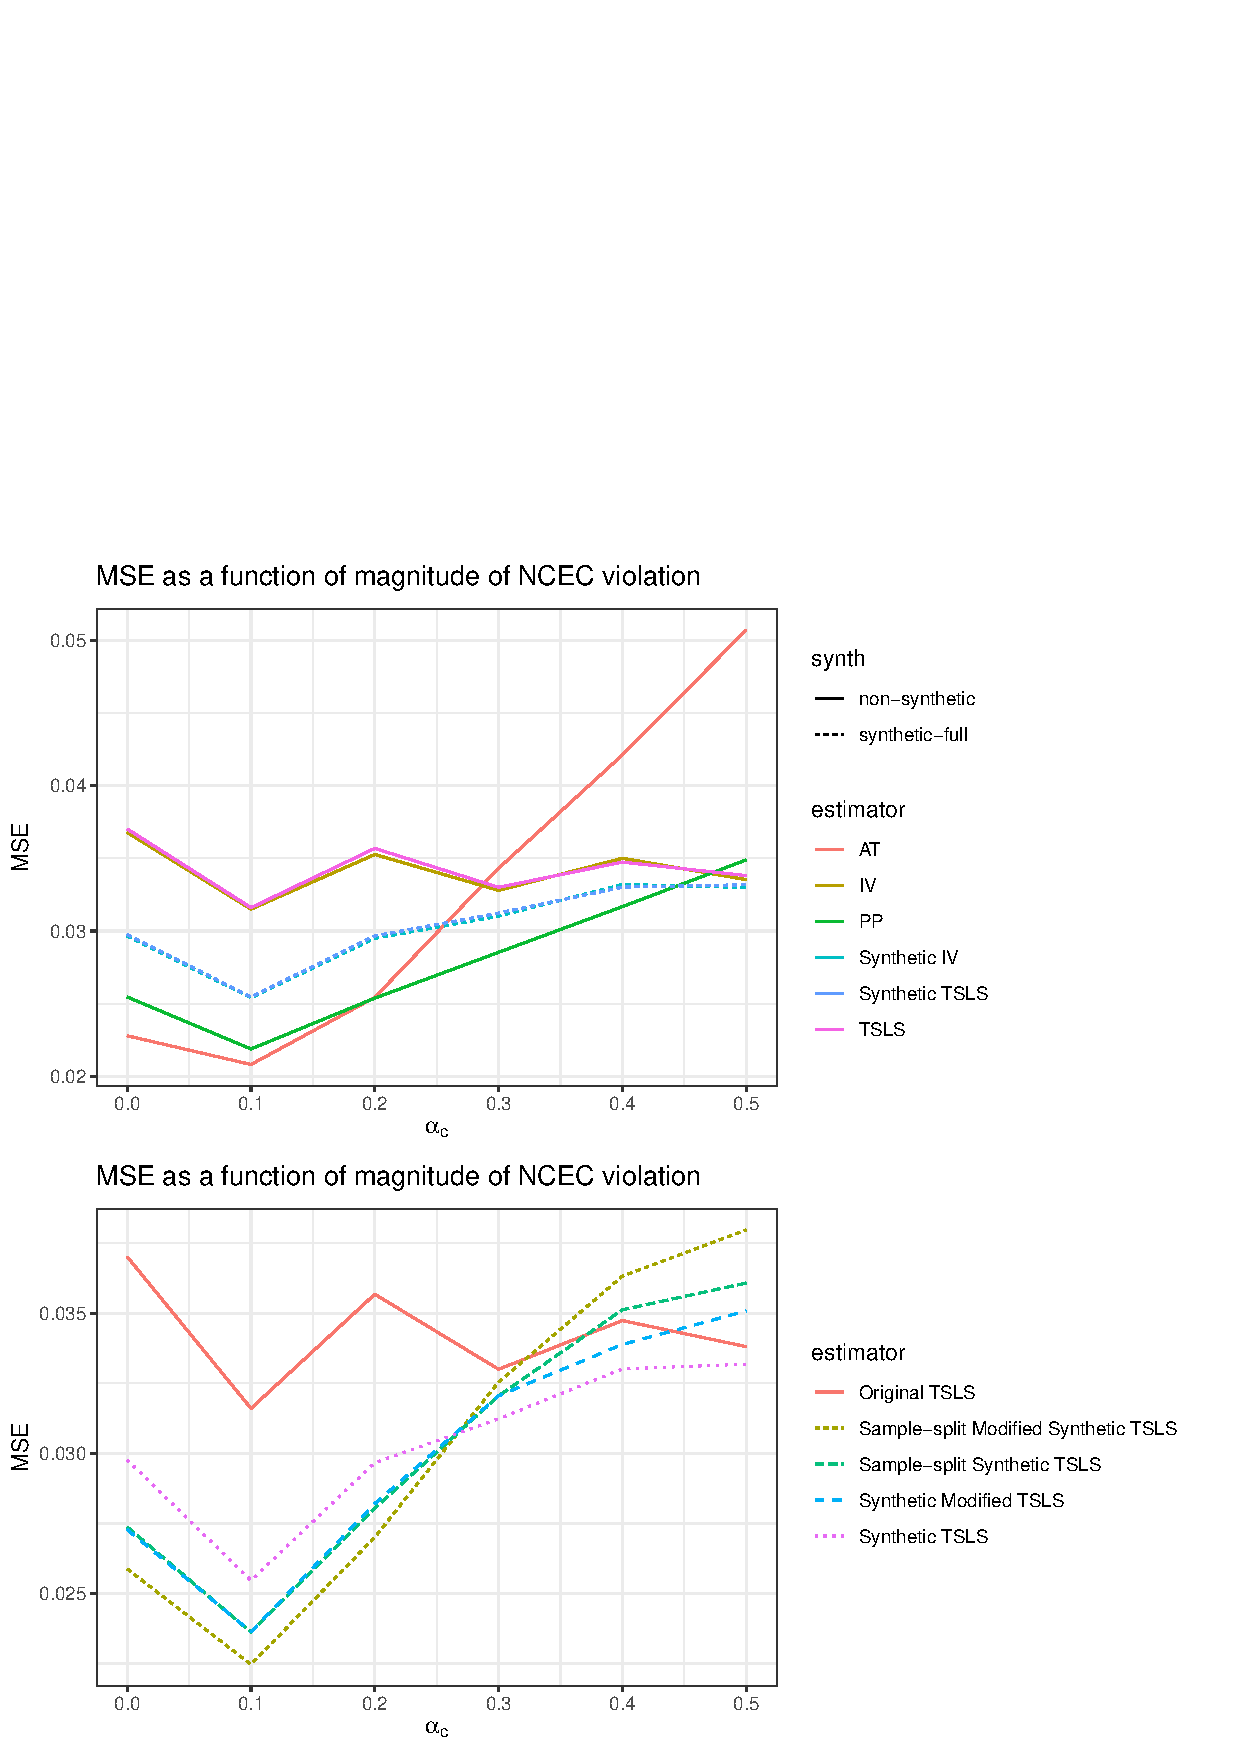
\includegraphics{mse_bias_var_for_n200_cp06.png}
\includegraphics[width =\textwidth]{figures/secondary-sim-mse-plot.png}
\end{tabular}\vspace{0.2in}
\caption{MSE, bias, and variance of the SCE with $\thetahat_0 = \thetahat\stsls$ compared to four of the candidate estimators for the CACE as $\eta$ changes in data-generating mechanism 1. The SCE includes information from all candidate estimators, but only four candidates are shown here. Sample sizes ($n = 200, 500, 1000$) are given in different facets.The y-axis for MSE and variance are given on the log-scale.}\label{sec-sim-pl}
\end{figure}

A similar robustness property was found in data-generating mechanism 2 (see Figure \ref{main-mse-p}. The SCE produces a sizable MSE reduction compare to $\thetahat\stsls$ when $\alpha_c$ is small and thus the bias and MSE of $\thetahat\sat$ and $\thetahat\saps$ are small. As the bias in $\thetahat\sat$ and $\thetahat\saps$ increase, the MSE of the synthetic estimator hovers at or near the MSE of $\thetahat\stsls$. The effects of creating a synthetic estimator are largest when compliance and sample size are both low (upper left panel in Figure \ref{main-mse-pl}, where the SCE is the best estimator when $\alpha_c = 0.5$). 
%
\begin{figure}
\centering
\begin{tabular}{c}
%\includegraphics{figure_1_correlations.eps}
%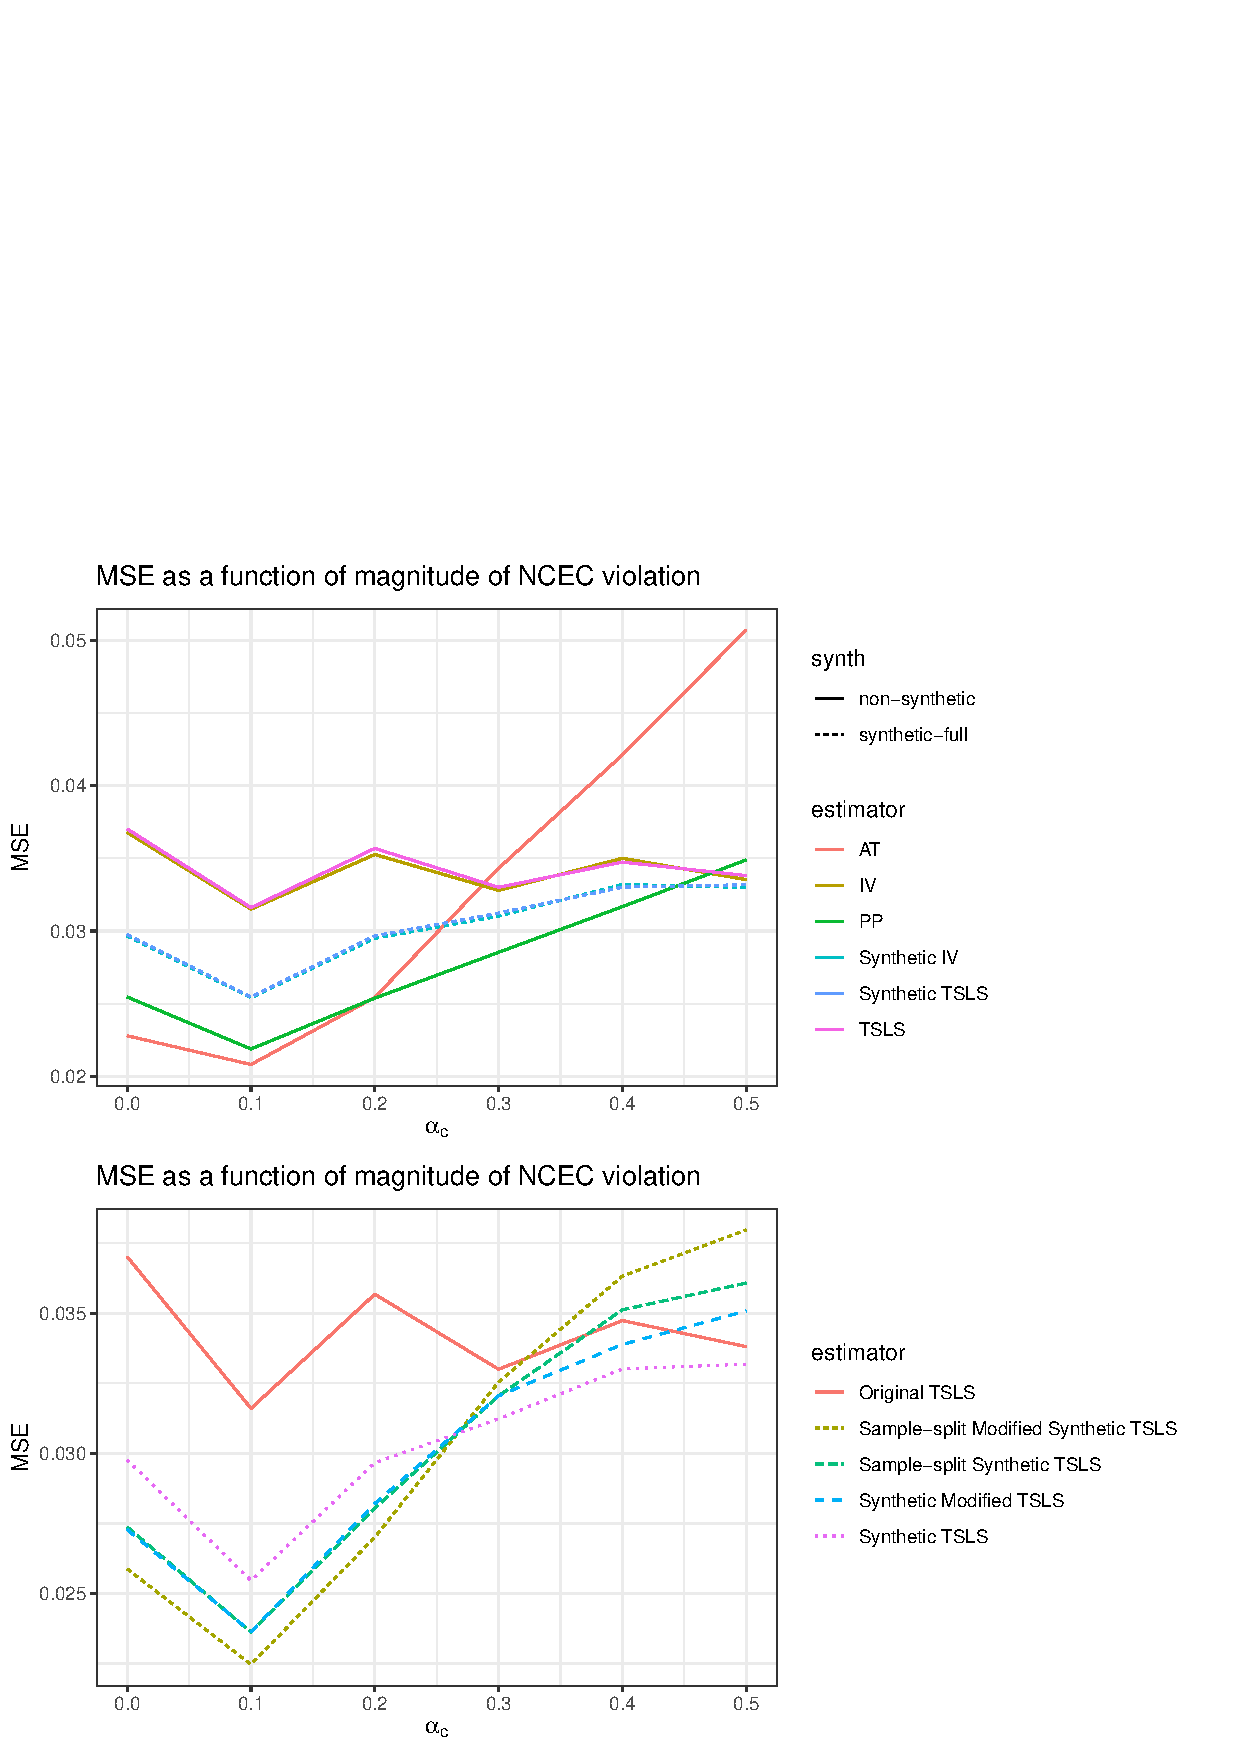
\includegraphics{mse_bias_var_for_n200_cp06.png}
\includegraphics[width =\textwidth]{figures/main-sim-mse-plot.png}
\end{tabular}\vspace{0.2in}
\caption{MSE of SCE with $\thetahat_0 = \thetahat\stsls$ compared to four of the candidate estimators for the CACE as $\alpha_c$ changes in data-generating mechanism 2. The SCE includes information from all candidate estimators, but only four candidates are shown here. Sample sizes of $n = 200, 500, 1000$ are given in the rows and compliance rates are given in the columns. Simulation parameters are set to $\gamma_c = 0, \lambda_n = \lambda_c = 1, \beta_0 = 0.41, \beta_1 = 2$. The y-axis is shown on the log-scale to highlight differences.}\label{main-mse-pl}
\end{figure}
%

\subsection{Effect of different bias estimates}
The performance of the SCE when using different estimates of the bias are shown in Figure \ref{sec-sim-pl2}. Three SCEs are shown, $\thraw, \thshr$, and $\thspl$, each with $\thetahat_0 = \thetahat\stsls$. These are compared to $\thetahat\stsls$ and the highest-bias, lowest-variance estimator, $\thetahat\sat$, which illustrates the relevant features. 

In the figure, $\thraw$ has performance closest to $\thetahat\stsls$ in terms of bias, variance, and MSE. As shown in Figure \ref{sec-sim-pl} as well, $\thraw$ took advantage of the other candidate estimators to decrease the variance of the TSLS estimator, while not incurring too much bias, even when the other estimators had a lot of bias. Using the alternative bias estimates loosened the relationship between $\thetahat_s$ and $\thetahat_0$, such that the SCEs took more advantage of the reduction in variance available from the other estimators, but at the same time suffered from higher bias when those estimators were more biased. In nearly all cases, $\thspl$ had the highest bias and lowest variance among the SCEs, with $\thshr$ falling between $\thspl$ and $\thraw$ in terms of both bias and variance. While $\thspl$ and $\thshr$ had markedly better performance than $\thraw$ when $\eta$ was close to 0 and all candidate estimators were unbiased, they also incurred upwards of 10-20\% bias in the extremes, and they even had worse performance than $\thetahat\stsls$ when sample size and $\eta$ were large ($n = 1000, \eta > 1$). 

\begin{figure}
\centering
\begin{tabular}{c}
%\includegraphics{figure_1_correlations.eps}
%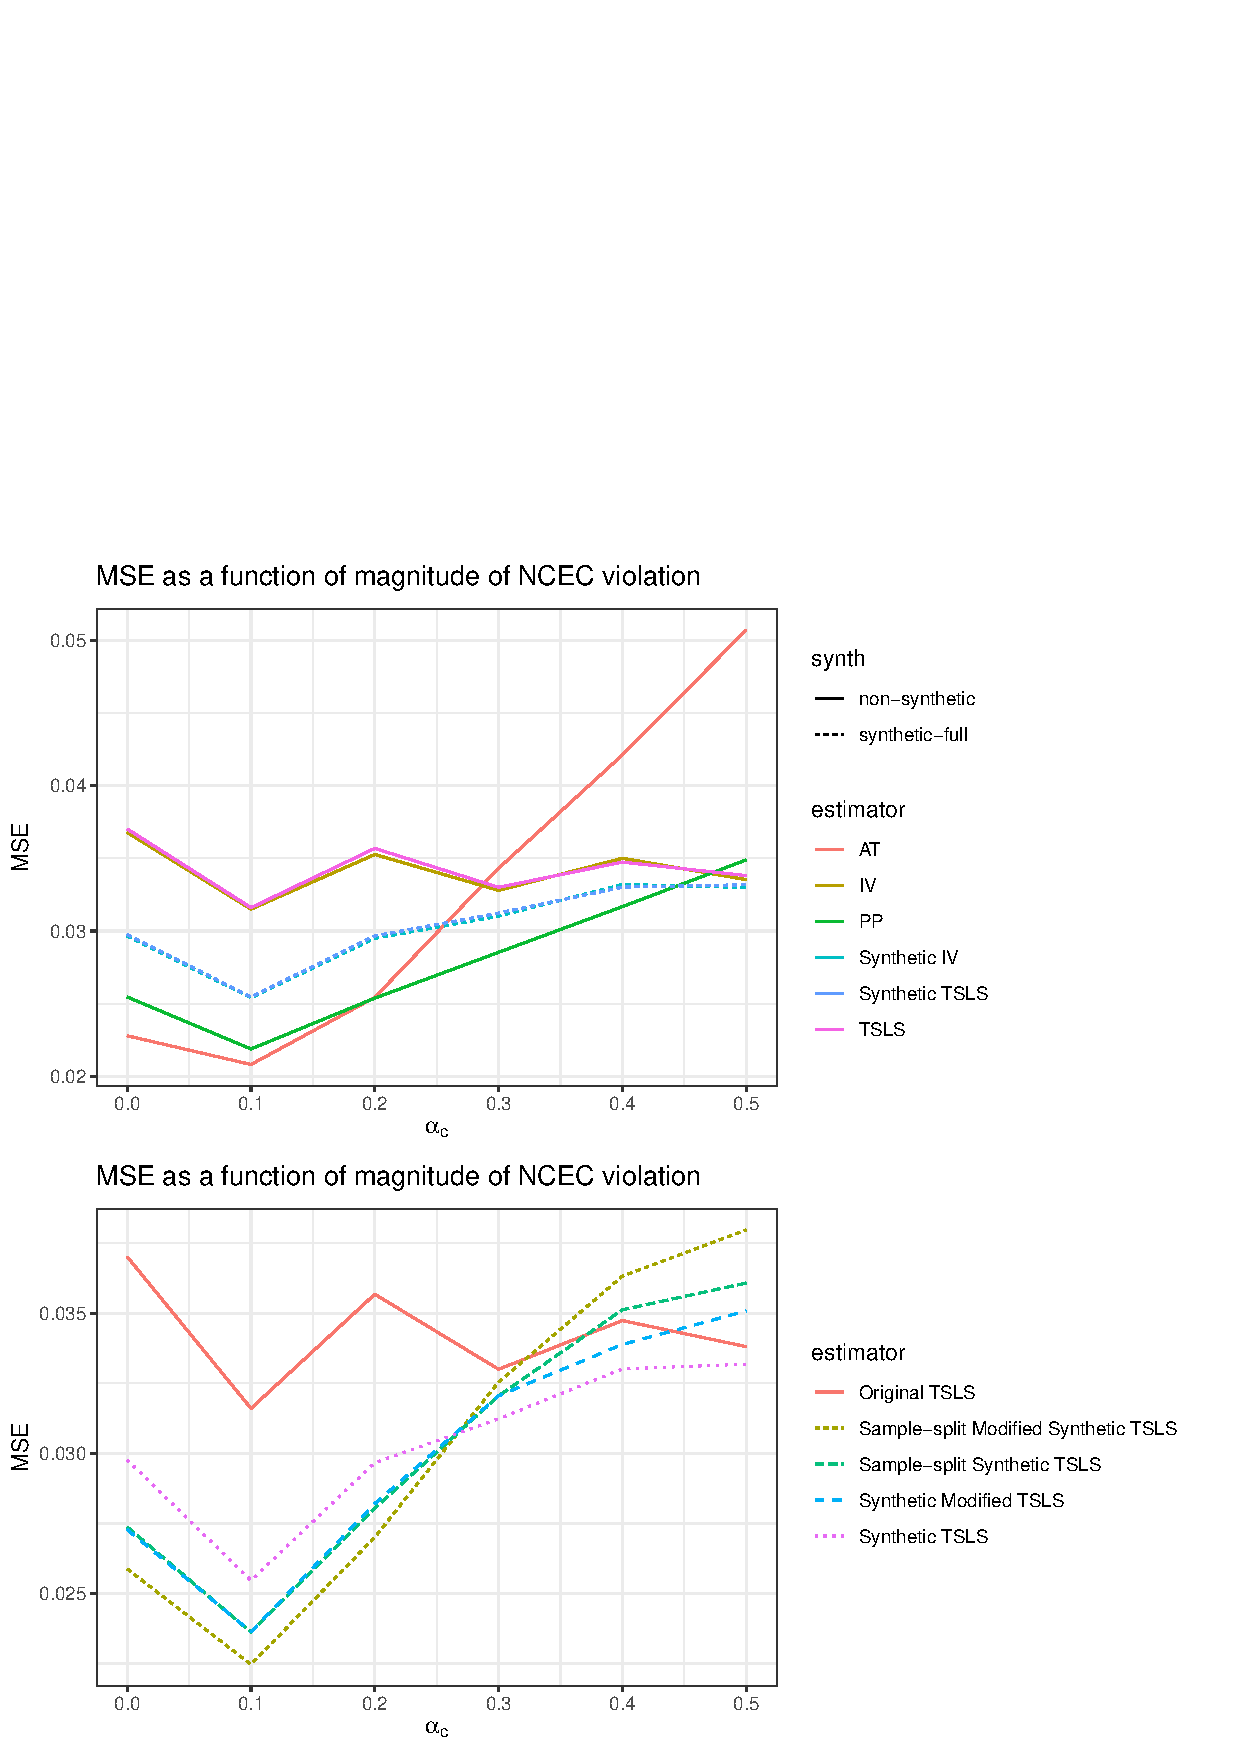
\includegraphics{mse_bias_var_for_n200_cp06.png}
\includegraphics[width =\textwidth]{figures/secondary-sim-synth-compare-plot.png}
\end{tabular}\vspace{0.2in}
\caption{MSE, bias, and variance of versions of the SCE with $\thetahat_0 = \thetahat\stsls$ and different bias estimates ($\bdhat_n$) as $\eta$ changes in data-generating mechanism 1. These are compared to $\thetahat\stsls$ and $\thetahat\sat$. The SCE includes information from all candidate estimators, but only four candidates are shown here. Sample sizes ($n = 200, 500, 1000$) are given in different facets.The y-axis for MSE and variance are given on the log-scale.}\label{sec-sim-pl2}
\end{figure}
%

\subsection{Confidence interval coverage}

\begin{figure}
\centering
\begin{tabular}{c}
%\includegraphics{figure_1_correlations.eps}
%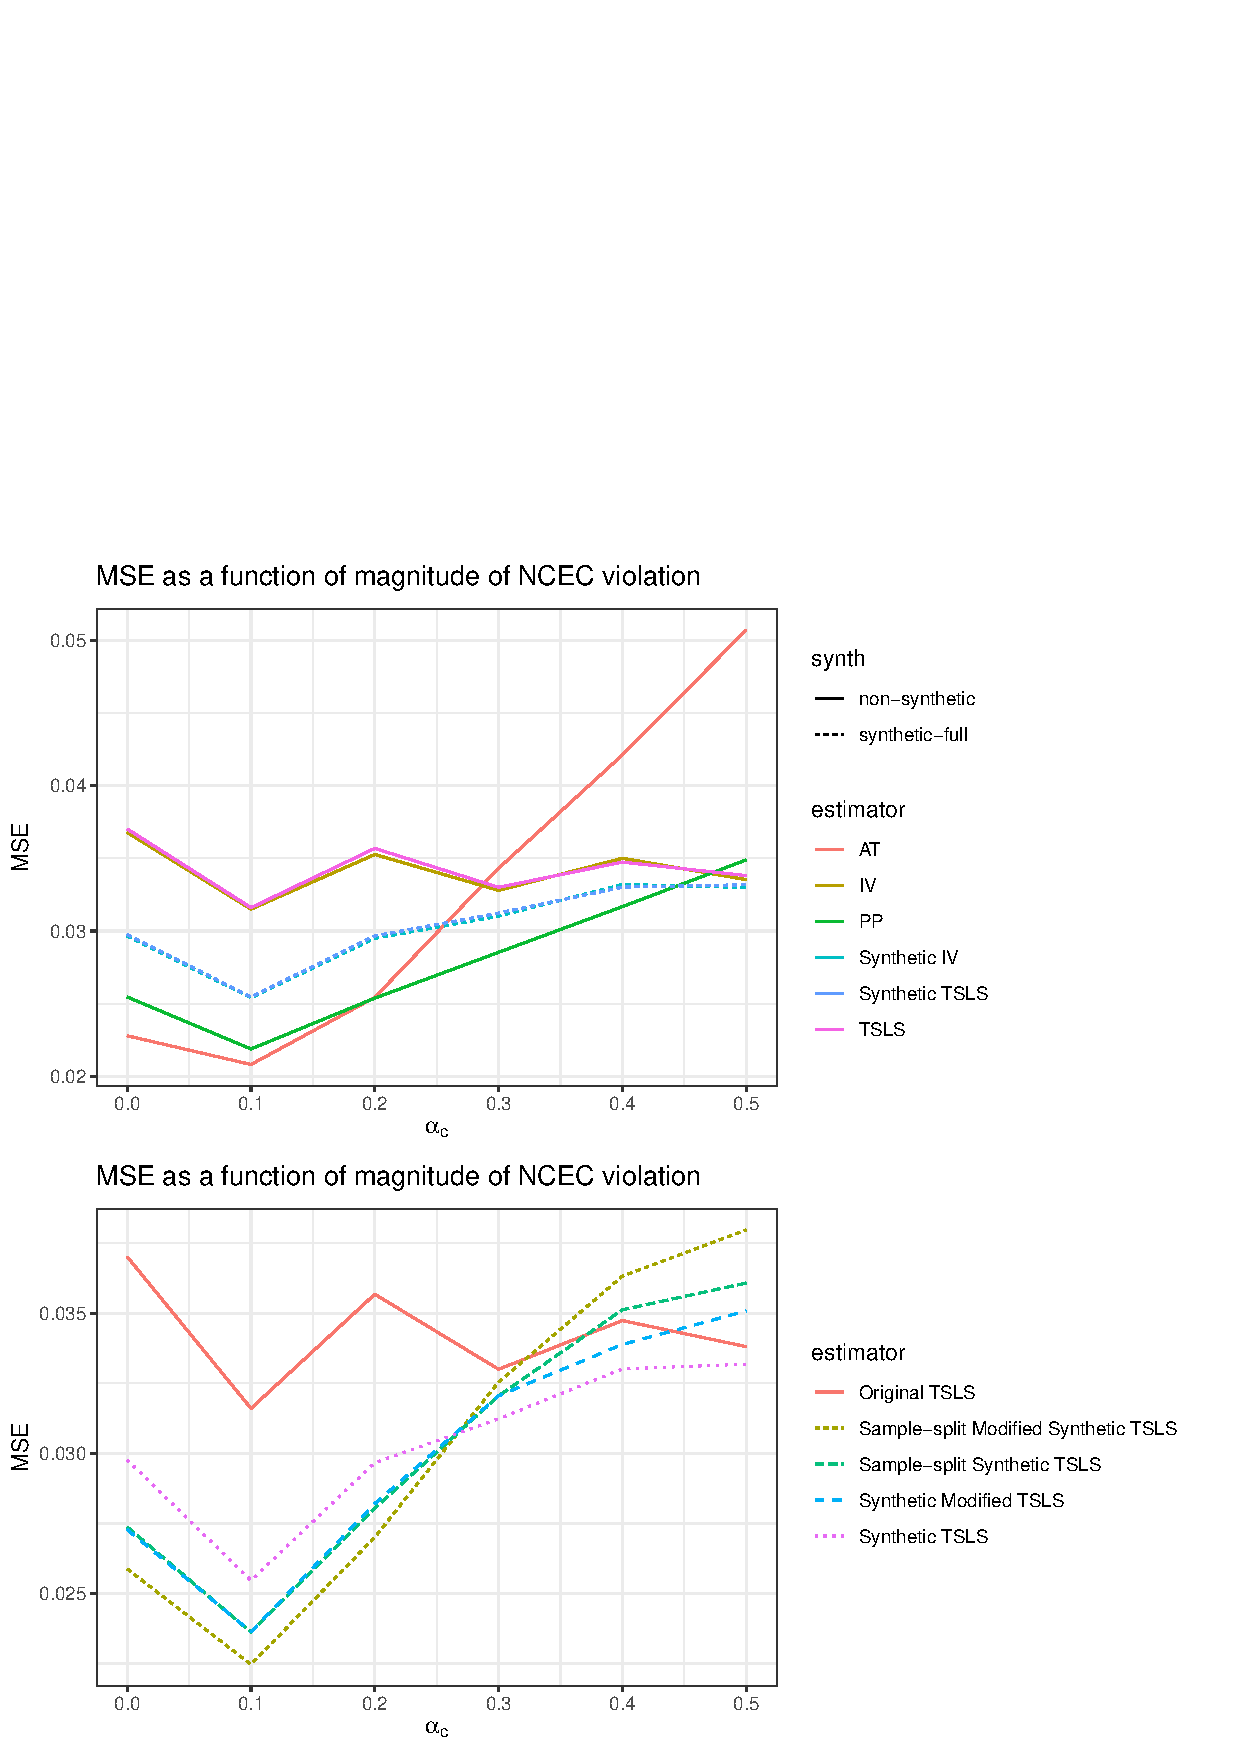
\includegraphics{mse_bias_var_for_n200_cp06.png}
\includegraphics[width =\textwidth]{figures/secondary-sim-synth-compare-plot.png}
\end{tabular}\vspace{0.2in}
\caption{MSE, bias, and variance of versions of the SCE with $\thetahat_0 = \thetahat\stsls$ and different bias estimates ($\bdhat_n$) as $\eta$ changes in data-generating mechanism 1. These are compared to $\thetahat\stsls$ and $\thetahat\sat$. The SCE includes information from all candidate estimators, but only four candidates are shown here. Sample sizes ($n = 200, 500, 1000$) are given in different facets.The y-axis for MSE and variance are given on the log-scale.}\label{sec-sim-pl2}
\end{figure}
\bibliography{compliance_refs}
\bibliographystyle{unsrtnat}

\end{document}

%\theta\right\}\sum_{j=1}^5\tdot_j(\bgamma_n)(\bgammahat_{nj} - \bgamma_{nj})\right],
%\] \\
%\end{split}\end{equation}
%\end{document}

